
%% bare_conf.tex
%% V1.4b
%% 2015/08/26
%% by Michael Shell
%% See:
%% http://www.michaelshell.org/
%% for current contact information.
%%
%% This is a skeleton file demonstrating the use of IEEEtran.cls
%% (requires IEEEtran.cls version 1.8b or later) with an IEEE
%% conference paper.
%%
%% Support sites:
%% http://www.michaelshell.org/tex/ieeetran/
%% http://www.ctan.org/pkg/ieeetran
%% and
%% http://www.ieee.org/

%%*************************************************************************
%% Legal Notice:
%% This code is offered as-is without any warranty either expressed or
%% implied; without even the implied warranty of MERCHANTABILITY or
%% FITNESS FOR A PARTICULAR PURPOSE! 
%% User assumes all risk.
%% In no event shall the IEEE or any contributor to this code be liable for
%% any damages or losses, including, but not limited to, incidental,
%% consequential, or any other damages, resulting from the use or misuse
%% of any information contained here.
%%
%% All comments are the opinions of their respective authors and are not
%% necessarily endorsed by the IEEE.
%%
%% This work is distributed under the LaTeX Project Public License (LPPL)
%% ( http://www.latex-project.org/ ) version 1.3, and may be freely used,
%% distributed and modified. A copy of the LPPL, version 1.3, is included
%% in the base LaTeX documentation of all distributions of LaTeX released
%% 2003/12/01 or later.
%% Retain all contribution notices and credits.
%% ** Modified files should be clearly indicated as such, including  **
%% ** renaming them and changing author support contact information. **
%%*************************************************************************


% *** Authors should verify (and, if needed, correct) their LaTeX system  ***
% *** with the testflow diagnostic prior to trusting their LaTeX platform ***
% *** with production work. The IEEE's font choices and paper sizes can   ***
% *** trigger bugs that do not appear when using other class files.       ***                          ***
% The testflow support page is at:
% http://www.michaelshell.org/tex/testflow/



	\documentclass[conference]{IEEEtran}
	\usepackage{subfigure}
% Some Computer Society conferences also require the compsoc mode option,
% but others use the standard conference format.
%
% If IEEEtran.cls has not been installed into the LaTeX system files,
% manually specify the path to it like:
% \documentclass[conference]{../sty/IEEEtran}





% Some very useful LaTeX packages include:
% (uncomment the ones you want to load)


% *** MISC UTILITY PACKAGES ***
%
%\usepackage{ifpdf}
% Heiko Oberdiek's ifpdf.sty is very useful if you need conditional
% compilation based on whether the output is pdf or dvi.
% usage:
% \ifpdf
%   % pdf code
% \else
%   % dvi code
% \fi
% The latest version of ifpdf.sty can be obtained from:
% http://www.ctan.org/pkg/ifpdf
% Also, note that IEEEtran.cls V1.7 and later provides a builtin
% \ifCLASSINFOpdf conditional that works the same way.
% When switching from latex to pdflatex and vice-versa, the compiler may
% have to be run twice to clear warning/error messages.






% *** CITATION PACKAGES ***
%
%\usepackage{cite}
% cite.sty was written by Donald Arseneau
% V1.6 and later of IEEEtran pre-defines the format of the cite.sty package
% \cite{} output to follow that of the IEEE. Loading the cite package will
% result in citation numbers being automatically sorted and properly
% "compressed/ranged". e.g., [1], [9], [2], [7], [5], [6] without using
% cite.sty will become [1], [2], [5]--[7], [9] using cite.sty. cite.sty's
% \cite will automatically add leading space, if needed. Use cite.sty's
% noadjust option (cite.sty V3.8 and later) if you want to turn this off
% such as if a citation ever needs to be enclosed in parenthesis.
% cite.sty is already installed on most LaTeX systems. Be sure and use
% version 5.0 (2009-03-20) and later if using hyperref.sty.
% The latest version can be obtained at:
% http://www.ctan.org/pkg/cite
% The documentation is contained in the cite.sty file itself.






% *** GRAPHICS RELATED PACKAGES ***
%
\ifCLASSINFOpdf
  % \usepackage[pdftex]{graphicx}
  % declare the path(s) where your graphic files are
  % \graphicspath{{../pdf/}{../jpeg/}}
  % and their extensions so you won't have to specify these with
  % every instance of \includegraphics
  % \DeclareGraphicsExtensions{.pdf,.jpeg,.png}
\else
  % or other class option (dvipsone, dvipdf, if not using dvips). graphicx
  % will default to the driver specified in the system graphics.cfg if no
  % driver is specified.
  % \usepackage[dvips]{graphicx}
  % declare the path(s) where your graphic files are
  % \graphicspath{{../eps/}}
  % and their extensions so you won't have to specify these with
  % every instance of \includegraphics
  % \DeclareGraphicsExtensions{.eps}
\fi
% graphicx was written by David Carlisle and Sebastian Rahtz. It is
% required if you want graphics, photos, etc. graphicx.sty is already
% installed on most LaTeX systems. The latest version and documentation
% can be obtained at: 
% http://www.ctan.org/pkg/graphicx
% Another good source of documentation is "Using Imported Graphics in
% LaTeX2e" by Keith Reckdahl which can be found at:
% http://www.ctan.org/pkg/epslatex
%
% latex, and pdflatex in dvi mode, support graphics in encapsulated
% postscript (.eps) format. pdflatex in pdf mode supports graphics
% in .pdf, .jpeg, .png and .mps (metapost) formats. Users should ensure
% that all non-photo figures use a vector format (.eps, .pdf, .mps) and
% not a bitmapped formats (.jpeg, .png). The IEEE frowns on bitmapped formats
% which can result in "jaggedy"/blurry rendering of lines and letters as
% well as large increases in file sizes.
%
% You can find documentation about the pdfTeX application at:
% http://www.tug.org/applications/pdftex





% *** MATH PACKAGES ***
%
%\usepackage{amsmath}
% A popular package from the American Mathematical Society that provides
% many useful and powerful commands for dealing with mathematics.
%
% Note that the amsmath package sets \interdisplaylinepenalty to 10000
% thus preventing page breaks from occurring within multiline equations. Use:
%\interdisplaylinepenalty=2500
% after loading amsmath to restore such page breaks as IEEEtran.cls normally
% does. amsmath.sty is already installed on most LaTeX systems. The latest
% version and documentation can be obtained at:
% http://www.ctan.org/pkg/amsmath





% *** SPECIALIZED LIST PACKAGES ***
%
%\usepackage{algorithmic}
% algorithmic.sty was written by Peter Williams and Rogerio Brito.
% This package provides an algorithmic environment fo describing algorithms.
% You can use the algorithmic environment in-text or within a figure
% environment to provide for a floating algorithm. Do NOT use the algorithm
% floating environment provided by algorithm.sty (by the same authors) or
% algorithm2e.sty (by Christophe Fiorio) as the IEEE does not use dedicated
% algorithm float types and packages that provide these will not provide
% correct IEEE style captions. The latest version and documentation of
% algorithmic.sty can be obtained at:
% http://www.ctan.org/pkg/algorithms
% Also of interest may be the (relatively newer and more customizable)
% algorithmicx.sty package by Szasz Janos:
% http://www.ctan.org/pkg/algorithmicx




% *** ALIGNMENT PACKAGES ***
%
%\usepackage{array}
% Frank Mittelbach's and David Carlisle's array.sty patches and improves
% the standard LaTeX2e array and tabular environments to provide better
% appearance and additional user controls. As the default LaTeX2e table
% generation code is lacking to the point of almost being broken with
% respect to the quality of the end results, all users are strongly
% advised to use an enhanced (at the very least that provided by array.sty)
% set of table tools. array.sty is already installed on most systems. The
% latest version and documentation can be obtained at:
% http://www.ctan.org/pkg/array


% IEEEtran contains the IEEEeqnarray family of commands that can be used to
% generate multiline equations as well as matrices, tables, etc., of high
% quality.




% *** SUBFIGURE PACKAGES ***
%\ifCLASSOPTIONcompsoc
%  \usepackage[caption=false,font=normalsize,labelfont=sf,textfont=sf]{subfig}
%\else
%  \usepackage[caption=false,font=footnotesize]{subfig}
%\fi
% subfig.sty, written by Steven Douglas Cochran, is the modern replacement
% for subfigure.sty, the latter of which is no longer maintained and is
% incompatible with some LaTeX packages including fixltx2e. However,
% subfig.sty requires and automatically loads Axel Sommerfeldt's caption.sty
% which will override IEEEtran.cls' handling of captions and this will result
% in non-IEEE style figure/table captions. To prevent this problem, be sure
% and invoke subfig.sty's "caption=false" package option (available since
% subfig.sty version 1.3, 2005/06/28) as this is will preserve IEEEtran.cls
% handling of captions.
% Note that the Computer Society format requires a larger sans serif font
% than the serif footnote size font used in traditional IEEE formatting
% and thus the need to invoke different subfig.sty package options depending
% on whether compsoc mode has been enabled.
%
% The latest version and documentation of subfig.sty can be obtained at:
% http://www.ctan.org/pkg/subfig




% *** FLOAT PACKAGES ***
%
%\usepackage{fixltx2e}
% fixltx2e, the successor to the earlier fix2col.sty, was written by
% Frank Mittelbach and David Carlisle. This package corrects a few problems
% in the LaTeX2e kernel, the most notable of which is that in current
% LaTeX2e releases, the ordering of single and double column floats is not
% guaranteed to be preserved. Thus, an unpatched LaTeX2e can allow a
% single column figure to be placed prior to an earlier double column
% figure.
% Be aware that LaTeX2e kernels dated 2015 and later have fixltx2e.sty's
% corrections already built into the system in which case a warning will
% be issued if an attempt is made to load fixltx2e.sty as it is no longer
% needed.
% The latest version and documentation can be found at:
% http://www.ctan.org/pkg/fixltx2e


%\usepackage{stfloats}
% stfloats.sty was written by Sigitas Tolusis. This package gives LaTeX2e
% the ability to do double column floats at the bottom of the page as well
% as the top. (e.g., "\begin{figure*}[!b]" is not normally possible in
% LaTeX2e). It also provides a command:
%\fnbelowfloat
% to enable the placement of footnotes below bottom floats (the standard
% LaTeX2e kernel puts them above bottom floats). This is an invasive package
% which rewrites many portions of the LaTeX2e float routines. It may not work
% with other packages that modify the LaTeX2e float routines. The latest
% version and documentation can be obtained at:
% http://www.ctan.org/pkg/stfloats
% Do not use the stfloats baselinefloat ability as the IEEE does not allow
% \baselineskip to stretch. Authors submitting work to the IEEE should note
% that the IEEE rarely uses double column equations and that authors should try
% to avoid such use. Do not be tempted to use the cuted.sty or midfloat.sty
% packages (also by Sigitas Tolusis) as the IEEE does not format its papers in
% such ways.
% Do not attempt to use stfloats with fixltx2e as they are incompatible.
% Instead, use Morten Hogholm'a dblfloatfix which combines the features
% of both fixltx2e and stfloats:
%
% \usepackage{dblfloatfix}
% The latest version can be found at:
% http://www.ctan.org/pkg/dblfloatfix




% *** PDF, URL AND HYPERLINK PACKAGES ***
%
%\usepackage{url}
% url.sty was written by Donald Arseneau. It provides better support for
% handling and breaking URLs. url.sty is already installed on most LaTeX
% systems. The latest version and documentation can be obtained at:
% http://www.ctan.org/pkg/url
% Basically, \url{my_url_here}.




% *** Do not adjust lengths that control margins, column widths, etc. ***
% *** Do not use packages that alter fonts (such as pslatex).         ***
% There should be no need to do such things with IEEEtran.cls V1.6 and later.
% (Unless specifically asked to do so by the journal or conference you plan
% to submit to, of course. )


% correct bad hyphenation here
\hyphenation{op-tical net-works semi-conduc-tor}

\usepackage{graphicx}
\begin{document}
%
% paper title
% Titles are generally capitalized except for words such as a, an, and, as,
% at, but, by, for, in, nor, of, on, or, the, to and up, which are usually
% not capitalized unless they are the first or last word of the title.
% Linebreaks \\ can be used within to get better formatting as desired.
% Do not put math or special symbols in the title.
\title{Extracted the style from the image\\with Deep Neural Network}


% author names and affiliations
% use a multiple column layout for up to three different
% affiliations
\author{\IEEEauthorblockN{Bingzhe Wu}
\IEEEauthorblockA{School of Mathmatical Science\\Peking University\\
	Email:wubingzhe@pku.edu.cn}
}


% conference papers do not typically use \thanks and this command
% is locked out in conference mode. If really needed, such as for
% the acknowledgment of grants, issue a \IEEEoverridecommandlockouts
% after \documentclass

% for over three affiliations, or if they all won't fit within the width
% of the page, use this alternative format:
% 
%\author{\IEEEauthorblockN{Michael Shell\IEEEauthorrefmark{1},
%Homer Simpson\IEEEauthorrefmark{2},
%James Kirk\IEEEauthorrefmark{3}, 
%Montgomery Scott\IEEEauthorrefmark{3} and
%Eldon Tyrell\IEEEauthorrefmark{4}}
%\IEEEauthorblockA{\IEEEauthorrefmark{1}School of Electrical and Computer Engineering\\
%Georgia Institute of Technology,
%Atlanta, Georgia 30332--0250\\ Email: see http://www.michaelshell.org/contact.html}
%\IEEEauthorblockA{\IEEEauthorrefmark{2}Twentieth Century Fox, Springfield, USA\\
%Email: homer@thesimpsons.com}
%\IEEEauthorblockA{\IEEEauthorrefmark{3}Starfleet Academy, San Francisco, California 96678-2391\\
%Telephone: (800) 555--1212, Fax: (888) 555--1212}
%\IEEEauthorblockA{\IEEEauthorrefmark{4}Tyrell Inc., 123 Replicant Street, Los Angeles, California 90210--4321}}




% use for special paper notices
%\IEEEspecialpapernotice{(Invited Paper)}




% make the title area
\maketitle

% As a general rule, do not put math, special symbols or citations
% in the abstract
\begin{abstract}

In the field of visual art,especially painting,humans have mastered the 
skill to create unique visual experience through composing a complex interplay
between the content and style of an image.In other area of computer vision such as object detection and recognition , Convolutional neural networks 
have recently enjoyed a great success in large-scale image recognition[1] which has become possible due to large public image repositories,such as ImageNet(Deng et al.,2009),and high-performance computing systems,such as GPUs
or large-scale distributed clusters(Dean et al.2012).In this project ,we use 
a neural representations to separate and recombine content and style of arbitrary images.This work also offers a algorithmic understanding of how
humans create and perceive artistic imagery.
\end{abstract}

% no keywords




% For peer review papers, you can put extra information on the cover
% page as needed:
% \ifCLASSOPTIONpeerreview
% \begin{center} \bfseries EDICS Category: 3-BBND \end{center}
% \fi
%
% For peerreview papers, this IEEEtran command inserts a page break and
% creates the second title. It will be ignored for other modes.
\IEEEpeerreviewmaketitle



\section{Introduction}
% no \IEEEPARstart
In this project ,we use a most powerful Deep Neural Networks in image processing called Convolutional Neural 
Networks .When Convolutional Neural Networks are trained on object recognition,they develop a representation of the image that makes object
information increasingly explicit along the processing hierarchy.Therefore,
along the processing hierarchy of the network,the input image is transformed
into representations that care about the actual content of the image compared
to its detailed pixel .In terms of this ,we can directly visualise the information each layer contains about the input image by reconstructing the image 
only from the feature maps in that layer.High layers in the network capture the high-level content in terms of objects and their arrangement in input image but do not constrain the exact pixel values of reconstruction.In contrast, reconstruction from the lower layers simply reproduce the exact
pixel values of the original image .In this project ,we refer to the feature 
responses in high layers of the networks as the content representation .


To obtain a representation of the style of an input image ,we use a featOn the ure
space originally designed to capture texture information.This feature space we used is built on top of the filter responses in each layer of the network
.It consists of the correlations between the different filter responses over the spatial extent of the feature maps.(See Implementation for details).By including the feature correlations of multiple layers,we obatain a multi-scale representation of the input image ,which captures its style information but not the details of content and its arrangement.

Again,we can visualise the information captured bt these style feature spaces built on different layers of the network by construction an image that matches the style representation of a given input image .Indeed reconstruction from the style features from the style features produce 
texturised versions of the input image that capture its general appearance in 
terms of color and localised structures.Moreover,the size and complexity of local image structures from the input image increases along the hierarchy,a result that can be explained by the increasing receptive field sizes and feature complexity.We refer to this multi-scale representation as style representation.

In this project ,we can manipulate both representation independently to produce new meaningful image.To demonstrate this work,we generate image mix 
the content and style representation from two different source images.In particular.

The images are synthesised by finding an image that simultaneously matches the
content representation of the photograph and the style representation of the
respective piece of art.While the global arrangement of the original photograph is preserved,the colors and local structures that compose the global scenery are provided by the artwork.Effectively,this renders the photograph in the style of the artwork,such that the apperance of the synthesised image resembles the work of art,even though it shows the same content as photograph.

Of course,image content and style cannot be completly disentangled.When synthesising an image that combine 
the content of one image whit the style of another image,there usually does not exist an image that perfectly 
matches both constrains at the same time.However,the loss function we minimise during image synthesis cotains
two terms for content and style respectively,that are well separated.We can therefore smoothly regulate 
the emphasis on either reconstructing the content or the style.

In my final project ,we set up an artificial system that achieves a separation
of image content from style,thus allowing to recast the content of one image in the style of any other image. We demonstrate this by creating new,artistic images that combine the style of several well-known paintings with the content of an arbitrarily chosen photograph that I take.In particular,we derive the neural representations for the content and style of an image from the feature responses of high-performing Deep Neural Networks trained 
on object recognition.

As outlined above, 

The rest of the report is organized as follows :Section 2 provides a background for CNN and VGG model,and also described the datasets for training model we used.Section 3 presents our described the 
method we used .Section 4 describes implementation details.Section5 shows our
experiment result.

\section{BACKGROUND}
\subsection{DATASETS}
ImageNet is a dataset of over 15 million labeled high-resolution images belong to roughly 22,000 categories.The images were collected from teh web and labeled by human labelers using Amazon's Mechanical Turk crowd-sourcing tool.Staring in 2010 ,as part of the Pascal Visual Object Challenge,an annual competition called the ImageNet Large-Scale Visual Recognition Challenge (ILSVRC) has benn held.ILSVRC uses a subset of ImageNet with roughly 1000
images in each of 1000 categories.In all,there are roughly 1.2 million training images,50,000 validation images,and 150,000 testing images.

ImageNet consists of variable-resolution images,while our system requires a constant input dimensionality .In our training process,we down-sampled the images to a fixed resolution of $256\times 256$.Given a image , we first rescaled 
the image such that the shorter side was of length 256,and then cropped out the central $256\times 256$ patch from the resulting image.We did not pre
-process the images in any other way,except for subtracting the mean activity over the training set from each pixel.
Then we use these picture for 
training a VGG19(see it in next subsection) model by Caffe(A deeplearning framework).

\subsection{CNN Basics}
Convolutional neural network (CNN) is first inspired by research in 
neuroscience.After over twenty years of convolution,CNN has been gaining 
more and more distinction in research fields,such as computer vision,pattern
recognition ,NLP.As a classical supervised learning algorithm,CNN employs 
a feedforward process for recognition and backward path for training.


A typical CNN is composed of two components : a feature extractor and a classifier . The feature extractor is used to filter input images into 
feature maps that represent various features of the image.These features may 
include corners,lines,circular arch,etc.,which are relatively invariant to
position shifting or distortions.The output of the feature extractor is a low-dimensional vector containing these features.This vector is then fed into the classifier ,which is usually based on traditional artificial neural 
networks.The purpose of this classifier is to decide the likelihood of 
categories that the input image might belong to.

A typical CNN is composed of multiple computation layers.For example,the feature extractor may consist of several convolutional layers and 
optional sub-sampling layers.Figure 1 illustrates the computation of a convolutional layer.The convolutional layer receives $N$ feature maps as input.Each input feature map is convolved by a shifting window is S,which 
is normally smaller than K.A totel of M output feature maps will form the 
set of input feature maps for the next convolutional layer.  

\begin{figure}[h]
	\centering
	{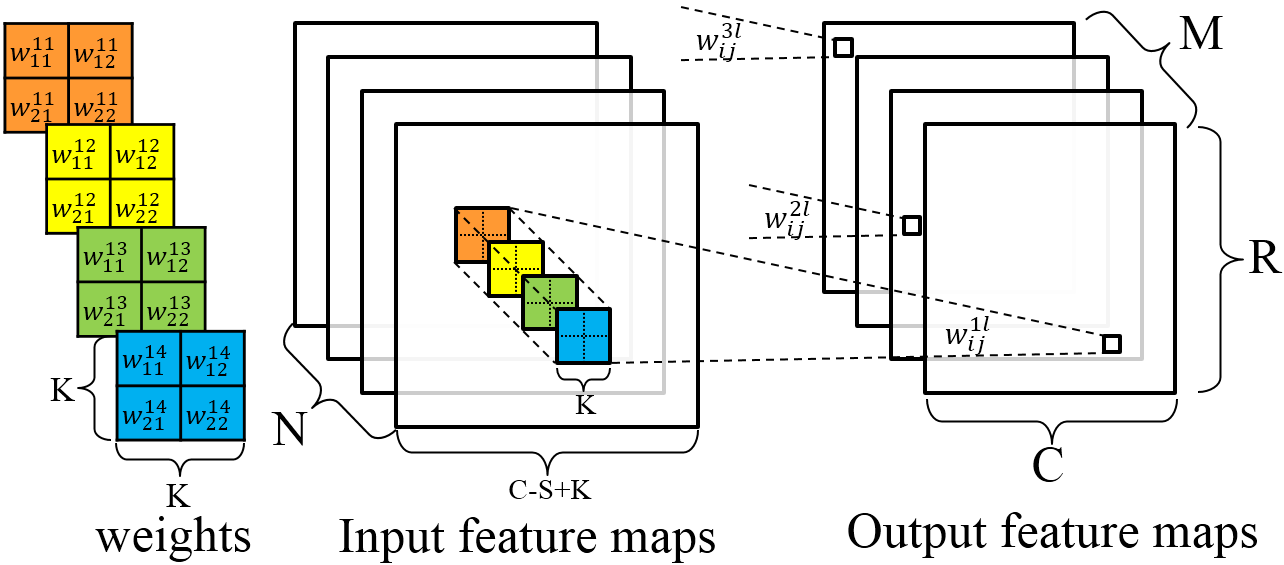
\includegraphics[width=0.8\linewidth]{convolve.png}}
	\caption{Graph of a convolutional layer}
%	\label{fig_convolve}
\end{figure}
\subsection{VGG Model}
\subsubsection{ARCHITECTURE}

VGG model is a convolutional neural network that rivals human performance 
on a common visual object recognition benchmark task and was introduced and 
extensively described in [10]. 

In this project ,we used VGG models for training.During training,the input
to this ConvNets is a fixed-size $224\times224$ RGB image.The only pre-processing we do is subtracting the mean RGB value,computed on the training set,from each pixel .The image is passed through a stack of 
convolution layers,where we use filters with a very small receptive field
:$3\times 3$(which is the smallest size to capture the notion of left/right,
up/down,center).In one of the configurations we also utilise $1\times1$ convolution filters,which can be seen as a linear transformation of the
input channels(followed by non-linearity).The convolutional stride is fixed 
to 1 pixel ; the spatial padding of conv.layer input is such that the spatial
resolution is preserved after convolution,i.e.the padding is 1 pixel for $3\times 3$ conv.layers.Spatial pooling is carried out by five max-pooling
layers,which follow some of the conv.layers(not all the conv.layers are followed by max-pooling).Max-pooling is performed over a $2\times 2$ pixel 
window,with stride 2.

A stack of convolutional layers (which has a different depth in different 
architectures) is followed by three Fully-Connected(FC) layers.However in our 
project ,teh full-connected layers was removed .

All hidden layers are equipped with the rectification(ReLU) non-linearity.
We note that none of our networks (except for one) contain Local Response
Normalisation (LRN) normalisation.

The Convnet we used in the project are shown in Figure2
\begin{figure}[h]
	\centering
	{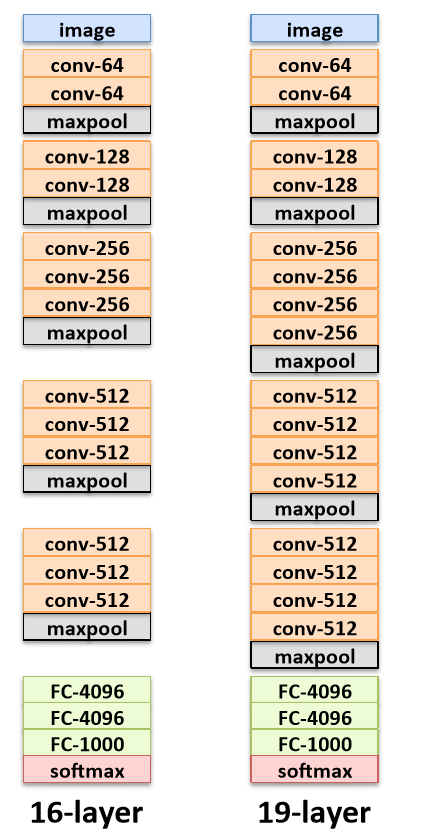
\includegraphics[width=0.8\linewidth]{vgg.png}}
	\caption{Graph of a convolutional layer}
	%	\label{fig_convolve}
\end{figure}
\section{Methods}
The results presented in our project were generated on the basis of 
the VGG-Model(see details in section 2).We used the feature space provide
by the 16 convolutional and 5 pooling layers of the 19 layer VGG-Network(
see the architecture in Figure 2).We do not use any of the fully connected layers.The model is publicly available and can be explored in the caffe-framework. For image synthesis we found that replacing the max-pooling operation by average pooling improves the gradient flow and one obtains slightly more appealing rsults,which is why the images shown were generated 
whit average pooling.

Generally each layer in the network defines a non-linear filter bank whose 
complexity increases with the position of the layer in the network .Hence a given input image $\overrightarrow{x}$is encoded in each layer of the CNN by the filter responses to that image.A layer with $N_l$ distinct filters has
$N_l$ feature maps each of size $M_l$,where $M_l$ is the height times 
the width of the feature maps. So the responses in a layer $l$ can be stored in a matrix $F^l \in R^{N_l\times M_l}$ where $F_{ij}^{l}$ is the 
activation of the $i^{th}$ filter at position $j$ in layer$l$
% An example of a floating figure using the graphicx package.
% Note that \label must occur AFTER (or within) \caption.
% For figures, \caption should occur after the \includegraphics.
% Note that IEEEtran v1.7 and later has special internal code that
% is designed to preserve the operation of \label within \caption
% even when the captionsoff option is in effect. However, because
% of issues like this, it may be the safest practice to put all your
% \label just after \caption rather than within \caption{}.
%
% Reminder: the "draftcls" or "draftclsnofoot", not "draft", class
% option should be used if it is desired that the figures are to be
% displayed while in draft mode.
%
%\begin{figure}[!t]
%\centering
%\includegraphics[width=2.5in]{myfigure}
% where an .eps filename suffix will be assumed under latex, 
% and a .pdf suffix will be assumed for pdflatex; or what has been declared
% via \DeclareGraphicsExtensions.
%\caption{Simulation results for the network.}
%\label{fig_sim}
%\end{figure}

% Note that the IEEE typically puts floats only at the top, even when this
% results in a large percentage of a column being occupied by floats.


% An example of a double column floating figure using two subfigures.
% (The subfig.sty package must be loaded for this to work.)
% The subfigure \label commands are set within each subfloat command,
% and the \label for the overall figure must come after \caption.
% \hfil is used as a separator to get equal spacing.
% Watch out that the combined width of all the subfigures on a 
% line do not exceed the text width or a line break will occur.
%
%\begin{figure*}[!t]
%\centering
%\subfloat[Case I]{\includegraphics[width=2.5in]{box}%
%\label{fig_first_case}}
%\hfil
%\subfloat[Case II]{\includegraphics[width=2.5in]{box}%
%\label{fig_second_case}}
%\caption{Simulation results for the network.}
%\label{fig_sim}
%\end{figure*}
%
% Note that often IEEE papers with subfigures do not employ subfigure
% captions (using the optional argument to \subfloat[]), but instead will
% reference/describe all of them (a), (b), etc., within the main caption.
% Be aware that for subfig.sty to generate the (a), (b), etc., subfigure
% labels, the optional argument to \subfloat must be present. If a
% subcaption is not desired, just leave its contents blank,
% e.g., \subfloat[].


% An example of a floating table. Note that, for IEEE style tables, the
% \caption command should come BEFORE the table and, given that table
% captions serve much like titles, are usually capitalized except for words
% such as a, an, and, as, at, but, by, for, in, nor, of, on, or, the, to
% and up, which are usually not capitalized unless they are the first or
% last word of the caption. Table text will default to \footnotesize as
% the IEEE normally uses this smaller font for tables.
% The \label must come after \caption as always.
%
%\begin{table}[!t]
%% increase table row spacing, adjust to taste
%\renewcommand{\arraystretch}{1.3}
% if using array.sty, it might be a good idea to tweak the value of
% \extrarowheight as needed to properly center the text within the cells
%\caption{An Example of a Table}
%\label{table_example}
%\centering
%% Some packages, such as MDW tools, offer better commands for making tables
%% than the plain LaTeX2e tabular which is used here.
%\begin{tabular}{|c||c|}
%\hline
%One & Two\\
%\hline
%Three & Four\\
%\hline
%\end{tabular}
%\end{table}


% Note that the IEEE does not put floats in the very first column
% - or typically anywhere on the first page for that matter. Also,
% in-text middle ("here") positioning is typically not used, but it
% is allowed and encouraged for Computer Society conferences (but
% not Computer Society journals). Most IEEE journals/conferences use
% top floats exclusively. 
% Note that, LaTeX2e, unlike IEEE journals/conferences, places
% footnotes above bottom floats. This can be corrected via the
% \fnbelowfloat command of the stfloats package.








% trigger a \newpage just before the given reference
% number - used to balance the columns on the last page
% adjust value as needed - may need to be readjusted if
% the document is modified later
%\IEEEtriggeratref{8}
% The "triggered" command can be changed if desired:
%\IEEEtriggercmd{\enlargethispage{-5in}}

% references section

% can use a bibliography generated by BibTeX as a .bbl file
% BibTeX documentation can be easily obtained at:
% http://mirror.ctan.org/biblio/bibtex/contrib/doc/
% The IEEEtran BibTeX style support page is at:
% http://www.michaelshell.org/tex/ieeetran/bibtex/
%\bibliographystyle{IEEEtran}
% argument is your BibTeX string definitions and bibliography database(s)
%\bibliography{IEEEabrv,../bib/paper}
%
% <OR> manually copy in the resultant .bbl file
% set second argument of \begin to the number of references





% that's all folks
\end{document}


